\documentclass[../report.tex]{subfiles}
\begin{document}

\section{Monitoring the System} \label{sec:monitor}
Monitoring the system is necessary to provide feedback to the user and to enable control of the charging process.

\subsection{Monitoring the Charge Current and Battery Voltage}
The battery voltage can be calculated from the measurement provided by $V_{ADC2}$:
\begin{equation}
    V_{ADC2}  = \frac{R_9}{R_8 + R_9} V_{Bat} \Rightarrow V_{Bat} = \left( 1 + \frac{R_8}{R_9} \right) V_{ADC1} = 3.9375 \cdot V_{ADC2}
\end{equation}
It is seen that the battery voltage is directly proportional to the measured voltage: $V_{Bat} \propto V_{ADC2}$.

The charge current, $i_{charge}$, can be calculated by the measurements $V_{ADC1}$ and $V_{ADC2}$. This is done by calculating the voltage over the shunt resistor $R_7$, after finding the voltage potentials at both sides:
\begin{align}
    V_{R_7} &= \left( 1 + \frac{R_5}{R_6} \right)V_{ADC1} - \left( 1 + \frac{R_8}{R_9} \right) V_{ADC2} = 3.9375 \cdot V_{ADC1} - 3.9375 \cdot V_{ADC2} \\
    \Rightarrow i_{charge} &= \frac{V_{R_7}}{R_7} = \frac{3.9375 \cdot V_{ADC1} - 3.9375 \cdot V_{ADC2}}{R_7} = 15.75\left( V_{ADC1} - V_{ADC2} \right) 
\end{align}
It is seen that the charge current is directly proportional to the difference in the two voltage measurements: $i_{charge} \propto \left( V_{ADC1} - V_{ADC2}  \right)$.

Thereby, both the battery voltage and charge current can be calculated very simply from the measured voltage potentials at the shunt resistor $R_7$:
\begin{align}
    V_{Bat} &= 3.9375 V_{ADC2}\\
    i_{charge} &= 15.75\left( V_{ADC1} - V_{ADC2} \right)
\end{align}

\subsection{Monitoring the State of Charge}
The state of charge can be represented as a function of the battery voltage, as shown in \cite{rsbattery}. The charging progress can be represented by the following equation:
\begin{equation} \label{eq:battery:state}
    \%_{Bat} = \frac{V_{Bat} - V_{Bat(0)}}{V_{Bat(Nominal)} - V_{Bat(0)}}
\end{equation}
In equation \ref{eq:battery:state} a linear characteristic is assumed between the battery charge in percentage and the battery voltage. During this report, the nominal voltage is $V_{Bat(Nominal)} = 1.5 [V]$, for a single battery, since this is the voltage at which the battery is fully recharged. The variable $V_{Bat(0)} = 1.1 [V]$ is the voltage at which the battery is fully decharged.

\subsection{Monitoring the Remaining Charge Time}
The following information about the battery is needed to calculate the remaining charge time: capacity, $Q$, and the charging current drawn by the battery.

%It is known that the maximal charging current for a battery is given by the following equation:
%\begin{equation}
%    i_{MAX} = Q \cdot C
%\end{equation}
Assuming a linear relationship between the charge current drawn by the battery and the charging time left in hours, the time left in hours can be calculated by the following:
\begin{equation}
    T_{LEFT} = \frac{Q}{i_{charge}}
\end{equation}

\subsection{Simulating the Monitoring of the Circuit}
The voltages measured by the two ADCs is now simulated to verify the design of the monitoring.

\begin{figure}[H]
    \centering
    \noindent\makebox[\textwidth][c]{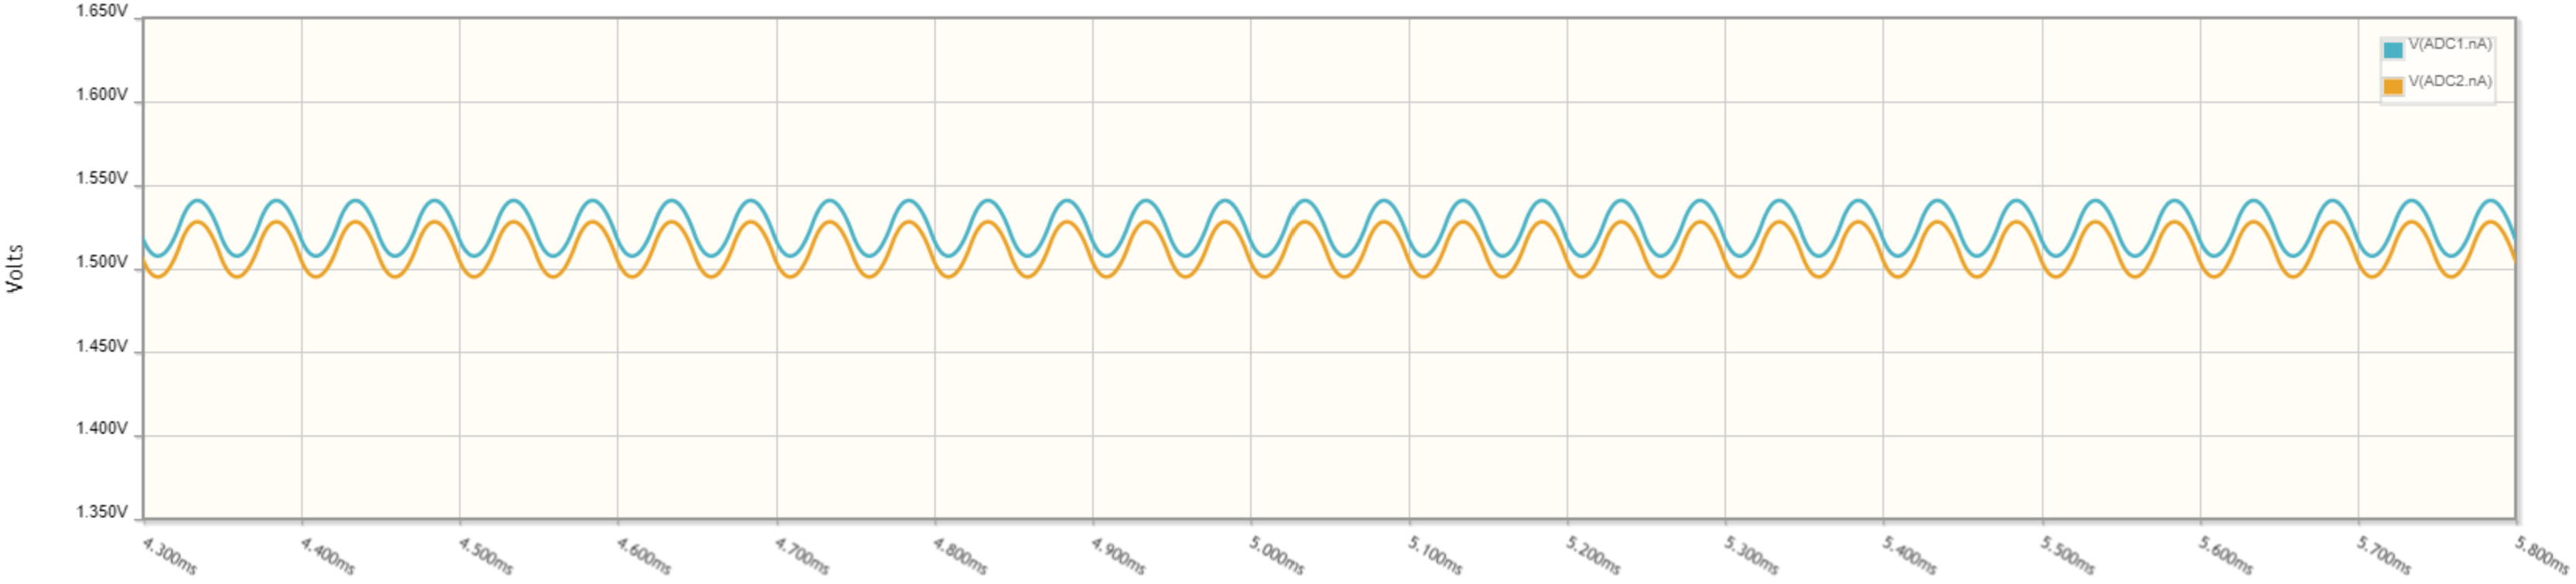
\includegraphics[width=1.2\textwidth]{figures/circuit/SIM_measure.png}}
    \caption{Simulation result of voltages read by ADC1 and ADC2. The blue line is the voltage read by ADC1, the yellow line is the voltage read by ADC2.}
    \label{fig:circuit:sim:monitoring}
\end{figure}

The verification of the design is done by two measurements. At time $t = 5.009 [ms]$ the voltages is $V_{ADC1} = 1.507 [V]$ and $V_{ADC2} = 1.495 [V]$. By utilizing the formulas above the charge current and battery voltage can be calculated:
\begin{align}
    t &= 5.009 [ms]\\
    V_{Bat}(t) &= 3.9375 \cdot V_{ADC2} = 5.88656 [V]\\
    i_{charge}(t) &= 15.75 \left( V_{ADC1} - V_{ADC2} \right) = 0.189 [A]
\end{align}
The actual battery voltage at $t = 5.009 [ms]$ is $5.885 [V]$ and the actual charge current is $0.196 [A]$, which is very close to the estimates. The actual values are read from the simulation results in \autoref{fig:circuit:sim:voltage} and \autoref{fig:circuit:sim:current}.\\
At the second timestamp $t = 5.134 [ms]$ the read voltages is $V_{ADC1} = 1.54048 [V]$ and $V_{ADC2} = 1.52768 [V]$.
\begin{align}
    t &= 5.134 [ms]\\
    V_{Bat}(t) &= 3.9375 V_{ADC2} = 6.0165 [V]\\
    i_{charge}(t) &= 15.75 \left( V_{ADC1} - V_{ADC2} \right) = 0.201 [A]
\end{align}
The actual values are read in  \autoref{fig:circuit:sim:voltage} and \autoref{fig:circuit:sim:current}, where it can be seen that the battery voltage at $t = 5.134 [ms]$ is $6.015 [V]$ and the actual charge current is $0.200 [A]$, which are also very close to the estimates.

\end{document}